\section{Design und Implementierung der Gegner und ihrer KI}\label{sec:enemiesAndAI}

Für die Entwicklung eines \textit{Schießspiels} (engl. \textit{Shooter}) ist neben der Spielersteuerung und der Waffen auch ein ausgereiftes Konzept für die Gegner unerlässlich. Damit das Spiel Spaß machen kann, müssen diese einerseits den Spieler fordern, dürfen aber andererseits nicht zu schwer zu besiegen sein.

Die Grundidee der Gegner sowie das Konzept für deren \textit{KI} wird in Abschnitt \ref{sec:enemyDesign} beschrieben. In Abschnitt \ref{sec:enemyImplementation} wird auf die Umsetzung der Idee in \textit{Unity} eingegangen. Schließlich wird in \ref{sec:pathfinding} auf die Implementierung des vom Gegner verwendeteten Wegfindungssystems eingegangen.

\subsection{Design der Gegner}
\label{sec:enemyDesign}

Das Design der Gegner ist für das Spiel von zentraler Bedeutung. Dabei wird Wert darauf gelegt, dass das Spiel nicht nur als \textit{Schießspiel}, sondern auch als \textit{Schleichspiel} (engl. \textit{Stealth game}) gespielt werden kann.

Im Folgenden werden das Verhalten der Gegner sowie Gegnervarianten beschrieben.

\subsubsection{Patrouillieren und Angriffsverhalten der Gegner}
\label{sec:enemyDesignAttack}

Die Gegner suchen bei Spielbeginn nicht aktiv nach dem Spieler, sondern haben ein Route, die sie zyklisch ablaufen. Diese Patrouille wird abgebrochen, sobald der Spieler entdeckt wird, was entweder deshalb passiert, weil der Spieler sich im Sichtfeld des Gegners befindet oder weil der Gegner diesen "hört" und sich zu ihm umdreht. Dabei bleibt der Gegner kurz stehen, bevor er zum Angriff übergeht. Dadurch ist der Übergang von Patrouille zu Angriff gut erkennbar und der Spieler hat mehr Zeit, auf den neuen Umstand zu reagieren, bevor er verfolgt wird.

Die Distanz, auf die der Gegner dem Spieler folgt, hängt mitunter von seiner Waffe ab: Hat er keine Waffe oder eine Nahkampfwaffe, versucht er, dem Spieler möglichst nahe zu kommen, um diese einsetzen zu können. Ein Gegner mit Fernkampfwaffe hat dagegen einen bevorzugten Abstand für den Angriff und verfolgt den Spieler nur, solange der Abstand zu diesem größer ist. Geht ihm die Munition aus, so legt er seine Waffe ab und geht zu einem Nahkampfangriff ohne Waffe über. 

Kommt der Gegner beim Verfolgen des Spielers in die Nähe eines anderen Gegners, schließt sich dieser der Verfolgung an, auch, wenn er den Spieler selbst nicht wahrgenommen hatte.

Verschwindet der Spieler aus dem Sichtfeld eines Gegners, so gibt dieser nach kurzer Zeit die Verfolgung auf und kehrt zu seiner Patroullenroute zurück.

\subsubsection{Gegnertypen}
\label{sec:enemyDesignTypes}

Um die Kämpfe abwechslungsreich zu gestalten, werden drei Gegnertypen entworfen, die unterschiedlich auf den Spieler reagieren und verschiedene Merkmale besitzen.

Der erste Gegnertyp, im folgenden als "leichter Gegner“ bezeichnet, wird als Nahkampfgegner konzipiert, der den Spieler erreichen muss, damit er Schaden anrichten kann. Dadurch hat der Spieler etwas länger Zeit, um zu reagieren, nachdem er entdeckt wurde. Damit er aber nicht zu leicht zu besiegen ist, ist der leichte Gegner beim Angriff etwas schneller als andere Gegner.

Der zweite Gegnertyp, der 
„mittelschwerer Gegner“ oder „Standardgegner“ genannt wird, ist dazu in der Lage, mit Fernkampfwaffen umzugehen und hat ein größeres Sichtfeld als der leichte Gegner, wodurch er eine größere Gefahr für den Spieler darstellt, da es schwerer ist, sich anzuschleichen.

Der dritte und letzte Gegnertyp ist am schwierigsten zu besiegen. Das wird einerseits durch bessere Werte bei den Charaktereigenschaften gewährleistet. Beispielsweise hat der „schwere Gegner“ ein größeres Sichtfeld, kann aus einer größeren Entfernung schießen und muss häufiger getroffen werden, bevor er stirbt. Andererseits hat der schwere Gegner zusätzliche Fähigkeiten, die ein intelligenteres Verhalten ermöglichen.

Zuallererst verfügt der schwere Gegner über eine höhere Zielsicherheit. Während die anderen Gegnertypen bei Verfolgung und Fernkampfangriffen auf den aktuellen Standort des Spielers zielen, ist der schwere Gegner dazu in der Lage, vorauszuberechnen, wohin sich der Spieler bewegt. Dadurch ist es für diesen schwieriger, Schüssen auszuweichen und den Gegner abzuhängen.

Das Entkommen wird durch eine hartnäckigere Verfolgung zusätzlich erschwert. Wenn der Spieler aus dem Sichtfeld eines Gegners verschwindet, wird er im Falle eines leichten oder mittelschweren Gegner nur zu dem Punkt verfolgt, an dem dieser ihn zuletzt gesehen hat. Der schwere Gegner ist für kurze Zeit dazu in der Lage, den Spieler auch dann weiter zu verfolgen, wenn sich dieser nicht im Sichtfeld befindet. Darauf wird in Kapitel \ref{sec:pathfindingIntegration} näher eingegangen.

Außerdem ist der schwere Gegner dazu in der Lage, andere Gegner des gleichen Typs auf die aktuelle Position des Spielers aufmerksam zu machen. Damit haben diese eine Art Schwarmintelligenz, die sich jedoch nur auf die Schwierigkeit des Spiels auswirkt, wenn mehrere Gegner von diesem Typ im Spiel sind.

\subsection{Implementierung des Gegnerverhaltens}
\label{sec:enemyImplementation}

Da das Gegnerverhalten relativ komplex ist, macht es einen großen Teil des Projekts aus. Deshalb wird in diesem Kapitel auf die wichtigsten Aspekte näher eingegangen.

Der Abschnitt \ref{sec:enemyImplementationTypes} behandelt dabei das Grundkonzept sowie die Struktur der Implementierung. Im Abschnitt \ref{sec:enemyImplementationFOV} wird auf das Sichtfeld der Gegner eingegangen, da dieses für die Weiterentwicklung des Spiels eine wichtige Rolle spielt (siehe \ref{sec:interfaceSerialization}). Der Abschnitt \ref{sec:enemyImplementationAwareness} befasst sich mit der Wahrnehmung der Gegner, wobei die Wahrnehmung von Geräuschen aufgrund der Komplexität des Audiosystems in Kapitel \ref{audio} separat behandelt wird.

\subsubsection{Implementierung der Gegnertypen}
\label{sec:enemyImplementationTypes}

Für die drei in \ref{sec:enemyDesignTypes} beschriebenen Gegnertypen gibt es jeweils ein \textit{Prefab} mit einem \textit{MonoBehaviour} für das Verhalten sowie einer eigenen Grafik zur Unterscheidung der Gegnertypen im Spiel.

In einer frühen Phase der Entwicklung wird das Verhalten als klassische Vererbungshierarchie umgesetzt, es gibt also die abstrakte Klasse \texttt{Enemy}, welche von der \texttt{Person} Klasse erbt und darunter die Klassen \texttt{EasyEnemy}, \texttt{BasicEnemy} und \texttt{HardEnemy}.

Das Verhalten, das alle Gegner gemeinsam haben, wird dabei in der abstrakten Klasse implementiert. Dazu gehört insbesondere xdie Patrouille, bei der eine Liste an Koordinaten zyklisch abgelaufen wird. Auch parametrisierbare Unterscheidungsmerkmale wie die Anzahl an Leben, die Größe des Sichtfeldes und die Geschwindigkeiten für Patrouille und Angriff befinden sich hier. Diese Variablen werden als \texttt{public} definiert, damit die Werte einfach direkt am \textit{Prefab} eingestellt werden können.

Die typspezifischen Fähigkeiten der Gegner werden dagegen in den Unterklassen implementiert. Das bedeutet, dass das Nahkampfverhalten in der \texttt{EasyEnemy}-Klasse definiert ist, das einfache Fernkampfverhalten in der \texttt{BasicEnemy}-Klasse und das intelligente Verhalten in der \texttt{HardEnemy}-Klasse.

Eine spätere Designanpassung, welche sich auf das Verhalten der Fernkampfgegner bei Fehlender Munition betrifft, ermöglicht eine Konsolidierung, da das Nahkampfverhalten nun für alle Gegnertypen benötigt wird und das intelligente Fernkampfverhalten des schweren Gegners nun als Erweiterung des Standardfernkampfverhaltens verstanden wird.

\begin{figure}[h]
 \centering
 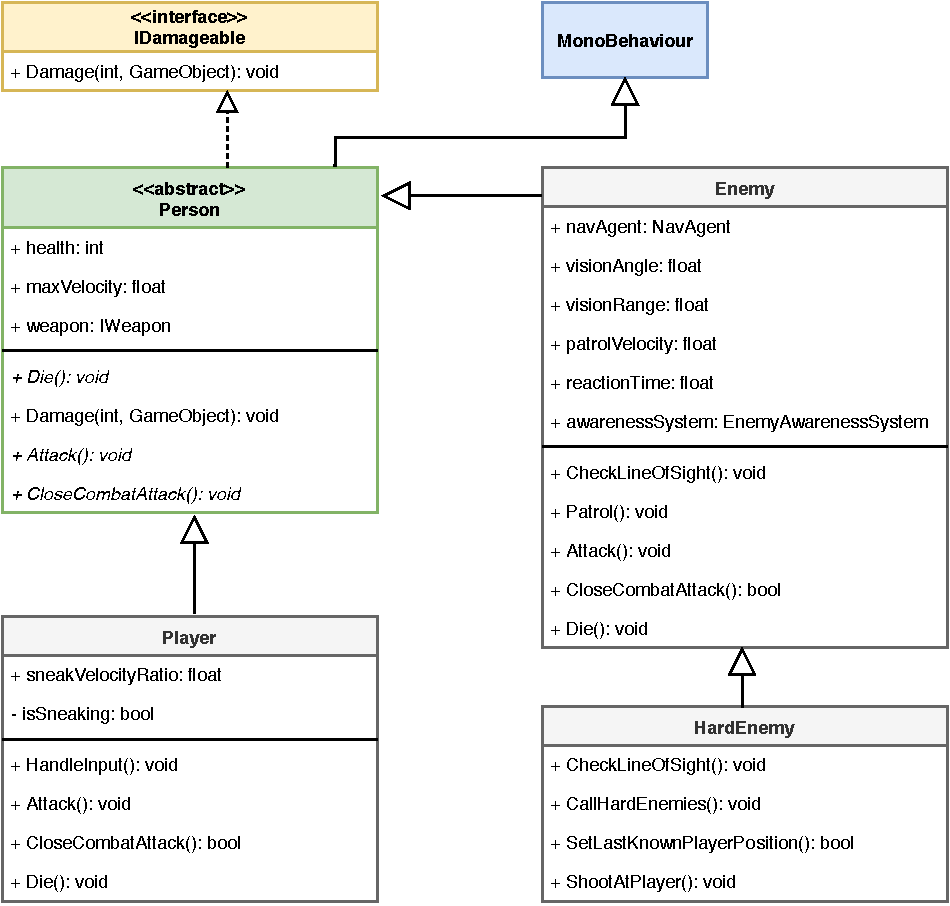
\includegraphics[width=0.835\linewidth]{diagrams/Person_Structure_reduced.pdf}
 \captionof{figure}[Datenstruktur der Charaktere]{UML-Klassendiagramm der Spielcharaktere in reduzierter Darstellung}
	\label{fig:charactersStructure}
\end{figure}


Die \texttt{Enemy}-Klasse ist deshalb nicht mehr abstrakt, sondern kann direkt an die \textit{Prefabs} der leichten und mittelschweren Gegner angehängt werden. Nur der schwere Gegner hat, wie in Abbildung \ref{fig:charactersStructure} zu sehen ist, noch eine eigene Unterklasse.

Diese Struktur lässt sich natürlich noch weiter verbessern. Es wäre beispielsweise möglich, die leichten und mittelschweren Gegner als eingeschränkte Varianten des schweren Gegners zu verstehen und auf dieser Grundlage alle Gegnertypen in der \texttt{Enemy}-Klasse zusammenzufassen. Die Unterschiede würden dann durch öffentliche Variablen festgelegt werden, d.h. die Gegnertypen würden sich nur noch an den Einstellungen am \textit{Prefab} unterscheiden.

Da die \texttt{Enemy}-Klasse ohnehin schon sehr umfangreich ist, wäre es eine sauberere Alternative, das Decorator-Entwurfsmuster zu verwenden. Wie in Kapitel \ref{sec:pathfindingIntegration} beschrieben, wird dieses für die Spielerverfolgung bereits eingesetzt. Die Schwarmintelligenz der schweren Gegner sowie die beiden Fernkampfvarianten könnten genauso umgesetzt werden. Das hätte den Vorteil, dass ohne Probleme neue Gegnerklassen oder neue Fähigkeiten der Gegner eingeführt werden können, ohne, dass an der bestehenden Klassenhierarchie etwas geändert werden muss.

\subsubsection{Das Sichtfeld der Gegner}
\label{sec:enemyImplementationFOV}

Das Sichtfeld des Gegners wird durch einen Blickwinkel und eine Reichweite definiert. Damit diese direkt am Prefab geändert werden können, sind diese Variablen \texttt{public}. Sie werden in der Methode \texttt{CheckLineOfSight()} benötigt, welche von der \texttt{Update()} Methode aufgerufen wird, um zu prüfen, ob sich der Spieler im Sichtfeld befindet.

Um die korrekte Implementierung des Sichtfeldes zu überprüfen, wird eine Visualisierung des Sichtfeldes eingebaut. Die einfachste Möglichkeit dafür ist die Verwendung der \textit{Gizmo}-Klasse \cite{Unity_Doc_Gizmo}, wie sie in Abbildung \ref{fig:fov1} zu sehen ist. Zur Fehlersuche ist diese Darstellung mithilfe eines Kreises für die Sichtweite und zweier Linien für den Blickwinkel zunächst ausreichend.

\begin{figure}[h]
 \centering
 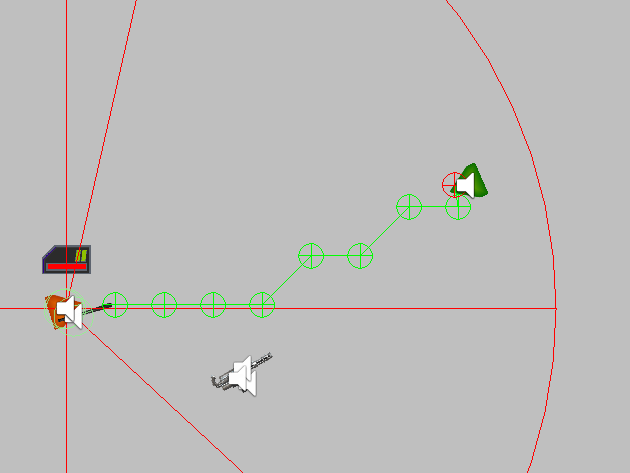
\includegraphics[width=0.835\linewidth]{pics/field-of-view_gizmo.png}
 \captionof{figure}[Visualisierung des Sichtfelds (Version 1)]{Visualisierung des Sichtfelds mit \textit{Gizmo}. Neben dem Sichtfeld werden hier auch die \textit{Gizmos} für Audioquellen und Pfadfindung angezeigt.}
	\label{fig:fov1}
\end{figure}

Mithilfe des \textit{Gizmos} kann im Unity Editor die Reaktion des Gegners auf ein Betreten des Sichtfeldes überprüft werden. Allerdings reagiert das \textit{Gizmo} nicht auf Objekte im Spielfeld, weshalb es so wirkt, als könnte der Gegner durch Wände hindurchsehen, was jedoch nicht der Fall ist. Hinzu kommt, dass Unity automatisch einen Fadenkreuz mitzeichnet, was die Übersichtlichkeit der Visualisierung beeinträchtigt.

Um dieses Problem zu lösen, gibt es mehrere Möglichkeiten. Eine davon wäre, das Sichtfeld mithilfe eines Lichtkegels mit entsprechendem Winkel und entsprechender Reichweite darzustellen. Das hätte den Vorteil, dass die Darstellung des Sichtfeldes automatisch auf Hindernisse im Spiel reagieren würde, aber den entscheidenden Nachteil, dass ein rechenintensives Lichtsystem eingeführt werden müsste, damit die Lichtkegel sichtbar werden \cite{Unity_Doc_Lighting}.

Die Alternative ist das Zeichnen einer Linie für den Umriss des Sichtfeldes. Dafür wird für jeden Winkel des Sichtfeldes mithilfe der Unity-Klasse \texttt{RayCast} überprüft, ob sich ein Hindernis im Sichtfeld befindet und welchen Abstand dieses zum Gegner hat \cite{Unity_Doc_RayCast}.

Da das Sichtfeld bei dieser Variante ohnehin als Linie dargestellt wird, bietet sich auch die Verwendung des \textit{LineRenderers} an \cite{Unity_Doc_LineRenderer}, wie sie in Abbildung \ref{fig:fov2} zu sehen ist. Das hat den Vorteil, dass das Sichtfeld ohne Zusatzaufwand auch im Spiel angezeigt werden kann und nicht, wie es beim \textit{Gizmo} der Fall war, nur im Unity-Editor.

\begin{figure}[h]
 \centering
 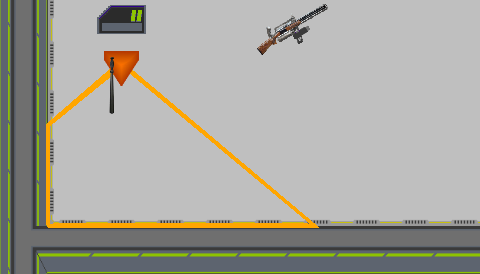
\includegraphics[width=0.835\linewidth]{pics/field-of-view_game.png}
 \captionof{figure}[Visualisierung des Sichtfelds (Version 2)]{Visualisierung des Sichtfelds mit LineRenderer unter Berücksichtigung von Hindernissen.}
	\label{fig:fov2}
\end{figure}

Die Farbe der Linie ist orange für leichte Gegner, rot für Standardgegner und dunkelrot für schwere Gegner. Ob das Sichtfeld visualisiert werden soll oder nicht kann am \texttt{PersonController} eingestellt werden.

\subsubsection{Implementierung des Wahrnehmungssystems}
\label{sec:enemyImplementationAwareness}

Die Wahrnehmung eines Gegners ist mit der Definition seines Sichtfeldes bei weitem nicht abgeschlossen. Die Anwesenheit des Spielers kann nämlich auch auf andere Art und Weise festgestellt werden.

Ein Aspekt ist, dass die Gegner den Spieler 
„hören“ können. Wie das Audiosystem genau funktioniert ist in Kapitel \ref{audio} beschrieben. Außerdem sind beispielsweise die schweren Gegner, wie bereits beschrieben wurde, dazu in der Lage, anderen Gegnern derselben Klasse die aktuelle Position des Spielers mitzuteilen.

Um die Wahrnehmung des Spielers durch den Gegner zu verwalten, wurde für diesen die Komponente \texttt{EnemyAwarenessSystem} implementiert. Diese hat eine Variable namens \texttt{awarenessLevel}, welche einen Wert zwischen null und hundert einnehmen kann und die aktuelle Wachsamkeit des Gegners wiederspiegelt. Externe Einflüsse auf die Wahrnehmung heben diesen Wert an. Dabei wird er beispielsweise durch Sichtkontakt sofort auf hundert angehoben, während er durch Geräusche je nach Lautstärke und Entfernung der Audioqulle unterschiedlich stark verändert wird. 

Die \texttt{Enemy}-Klasse ruft einmal pro \texttt{Update()}-Aufruf die Methode \texttt{IsAboveThreshold} der zugehörigen \texttt{AwarenessSystem}-Komponente ab. Diese Methode gibt an, ob das \texttt{awarenessLevel} über dem Wert der öffentlichen, am Gegner-\textit{Prefab} konfigurierbaren Variable \texttt{attackThreshold liegt.}

Dieser Schwellwert legt fest, wann sich der Status des Gegners ändert: Befindet sich das aktuelle \texttt{awarenessLevel} unter diesem Wert, so patrouilliert der Gegner; befindet es sich über dem Schwellwert, so greift der Gegner den Spieler an.

Damit der Gegner den Spieler nicht dauerhaft weiter verfolgt, gibt es eine Abklingzeit, welche in der Variable \texttt{awarenessCooldown} gespeichert ist. Sobald der Spieler sich nicht mehr im Sichtfeld des Gegners befindet, wird, sofern sie nicht bereits läuft, die \textit{Coroutine} \texttt{AwarenessCooldown()} gestartet, welche das \texttt{awarenessLevel} nach und nach senkt. Sobald der Wert des \texttt{awareness\-Level} wieder unter dem des \texttt{attackThreshold} liegt, wird die Verfolgung abgebrochen.

Die Schwarmintelligenz des schweren Gegners knüpft direkt an das Wahrnehmungssystem an. Hat ein schwerer Gegner den Spieler entdeckt, so wird aus dem \texttt{PersonController}, welcher für die Instanziierung der Gegner zuständig ist, eine Liste der schweren Gegner abgerufen, welche beim \texttt{PersonController} registriert sind. Für jeden dieser Gegner wird das \texttt{awarenessLevel} auf den maximalen Wert gesetzt und die \texttt{lastKnownPlayerPosition} des Gegners auf die aktuelle Position des Spielers. Die schweren Gegner konvergieren daraufhin auf diese Position, aber da der Cooldown für alle Gegner, die nicht in Sichtweite sind, sofort eingeleitet wird, kann es je nach Levelaufbau dennoch für den Spieler möglich sein, zu entkommen, ohne alle schweren Gegner auf einmal bekämpfen zu müssen.

\subsubsection{Implementierung des Gegnertods}
\label{sec:enemyImplementationDeath}

Wird der Gegner durch den Spieler oder durch Fehlschüsse anderer Gegner getroffen, so verliert dieser Lebenspunkte. Ist die Zahl der Lebenspunkte kleiner oder gleich null, so stirbt er.

Der Tod wird folgendermaßen implementiert: Zuerst wird der \textit{Collider2D} des Gegners deaktiviert, sodass er andere Charaktere nicht mehr blockiert. Das Ziel seines \textit{NavAgents} wird auf null gesetzt, sodass er stehen bleibt. Die Waffe wird abgelegt und dann wird durch den \texttt{PersonController} eine Ausblendung eingeleitet, welche damit endet, dass das Spieleobjekt des Gegners zerstört wird. Der \texttt{PersonController} wird deshalb in den Prozess mit einbezogen, weil die Gegner bei ihm registriert sind und damit bei der Weiterentwicklung des Spiels ohne großen Aufwand eine Wiederbelebung implementiert werden kann.

\subsection{Entwicklung des Wegfindungssystems für die Gegner}\label{sec:pathfinding}
Ein zentraler Bestandteil zur Realisierung der künstlichen Intelligenz der Gegner im Spiel ist das Wegfindungssystem. Dieses soll es Gegnern ermöglichen zur Laufzeit des Spiels dynamisch Pfade im Spiellevel zu vorgegebenen Zielpunkten kalkulieren zu lassen und diese schließlich zu traversieren. Ziel des Wegfindungssystems ist es, dass Gegner oder gegebenenfalls auch andere Spielobjekte nur einen Zielpunkt auf dem Level festlegen müssen und die restlichen Berechnungen unabhängig vom Spielobjekt durchgeführt werden.

Hierzu wird zunächst in Abschnitt \ref{sec:pathfindingConcept} das Zusammenspiel und Konzept der zentralen Komponenten genau dargestellt.
Anschließend werden in den Kapiteln \ref{sec:pathfindingAlgo}, \ref{sec:pathProcessing} und \ref{sec:pathCaching} der konkrete Pfadfindealgorithmus, die Pfadnachbearbeitung und die integrierte temporäre Pfadspeicherung zur Performanzverbesserung genauer erläutert. In Kapitel \ref{sec:pathfindingIntegration} wird schließlich behandelt, wie das System bei den Gegnern integriert wird, sodass sie sich im Level fortbewegen und dem Spieler folgen können.

\subsubsection{Grundlegendes Konzept des Systems}\label{sec:pathfindingConcept}
Beim Design der Architektur für das Pfadfindesystem dient die bereits in Unity integrierte Navigationsmechanik \cite{Unity_Doc_Navmesh} als grundlegendes Vorbild. Unity unterteilt die Logik in erster Linie in zwei Komponenten, nämlich in ein \textit{NavMesh} und eine beliebige Anzahl sogenannter Agenten. Das \textit{NavMesh} ist der zentrale Dreh- und Angelpunkt für die Navigation im Level. Es unterteilt das Level abhängig von nicht-passierbaren Hindernissen in begehbare Sektoren in Form von Polygonen und bietet die Funktionalität zur Pfadberechnung auf dem Level. In der Regel existiert pro Szene maximal ein \textit{NavMesh}. Die Agentenkomponente kann zu beliebigen Spielobjekten hinzugefügt werden, die schließlich das \textit{NavMesh} zur Fortbewegung nutzen sollen. In dieser Komponente kann das Bewegungsverhalten außerdem zum Beispiel in Form der Beschleunigung oder Maximalgeschwindigkeit eingestellt werden.

Theoretisch eignet sich das bereits in Unity integrierte System auch für diesen konkreten Anwendungsfall, jedoch ermöglicht eine eigene Implementierung eine optimale Anpassung des Pfadfindungssystems auf die in Kapitel \ref{sec:levelStructure} beschriebene Levelstruktur, da sich der Graph für den Wegfindungsalgorithmus effizient zur Laufzeit berechnen lässt, wie in diesem Kapitel noch genauer erläutert wird. Ebenfalls lässt sich das System so problemlos für zusätzliche Anwendungsfälle im Spiel nutzen. So wird es unter anderem auch zur Entfernungsberechnung von Geräuschen eingesetzt (siehe Kapitel \ref{sec:gegnerreaktionaufaudio}). Aufgrund dessen fällt die Entscheidung darauf, ein eigenständiges Pfadfindungssystem zu realisieren.

\begin{figure}[h]
 \centering
 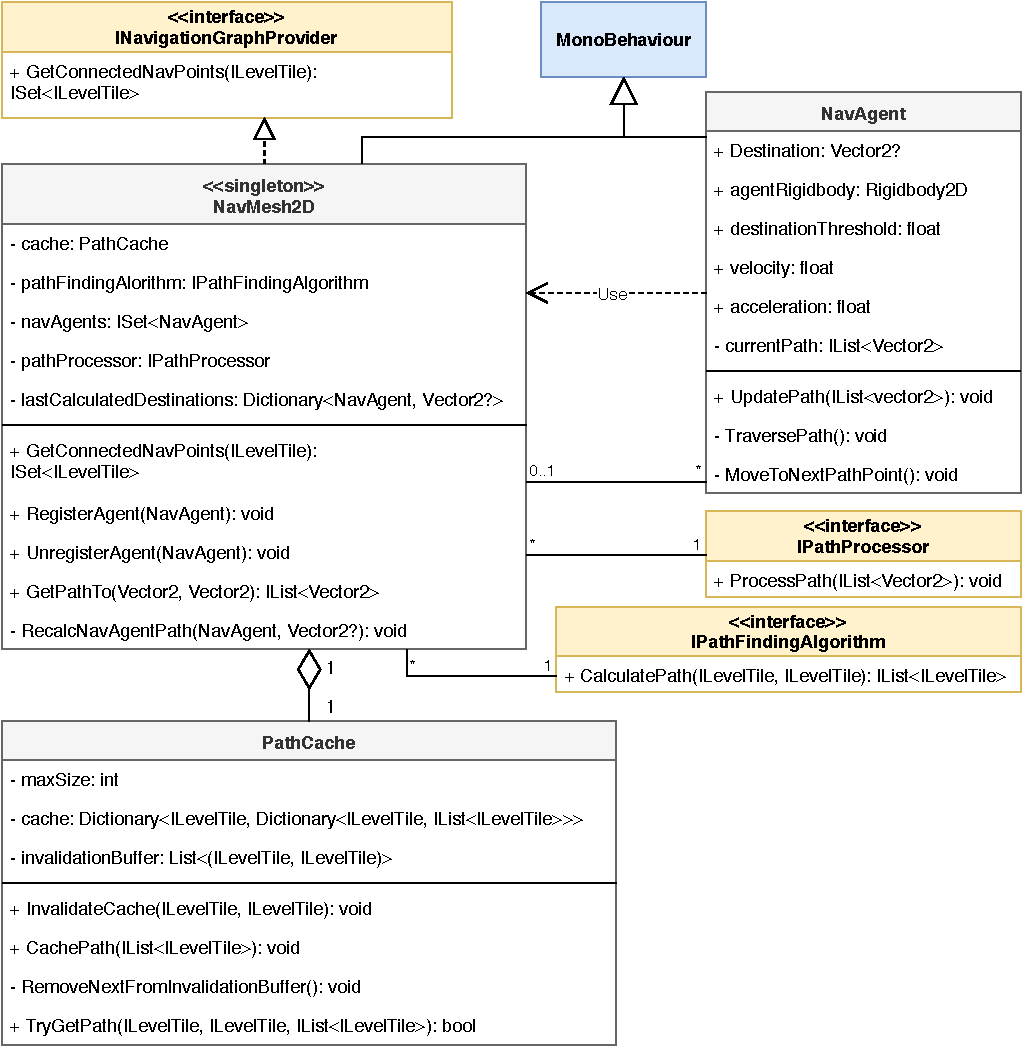
\includegraphics[width=0.835\linewidth]{diagrams/Pathfinding_Structure_reduced.pdf}
 \captionof{figure}[Aufbau des Pfadfindungssystems]{UML-Klassendiagramm der wichtigsten Komponenten des Pfadfindungssystems in vereinfachter Darstellung.}
	\label{fig:pathfinding_structure}
\end{figure}

In der Verwendung unterscheidet sich die Agentenkomponente (\texttt{NavAgent}) kaum vom  Pendant der Unity-Engine, wie in Abbildung \ref{fig:pathfinding_structure} zu sehen ist. Über die \texttt{Destination} lässt sich der momentane Zielpunkt des \texttt{NavAgent} konfigurieren, wobei ein Wert von \texttt{null} indiziert, dass der Agent sich nicht bewegen soll. Ebenso lässt sich die Maximalgeschwindigkeit und die Beschleunigung einstellen. Im Falle der Gegner ist der \texttt{NavAgent} eine Komponente des Spielobjekts und das zentrale Skript der Gegner übernimmt dessen Konfiguration. Der \texttt{NavAgent} hält zudem eine Referenz auf den momentanen Pfad in Form einer Liste von Punkten und traversiert diesen abschnittsweise. Die \texttt{destinationThreshold} definiert dabei, wie nahe sich der Agent an den nächsten Pfadpunkt annähern muss, dass dieser als erreicht gewertet und aus dem aktuellen Pfad entfernt wird. Die Fortbewegung wird dabei durch Anwendung von physikalischen Kräften am \textit{Rigidbody2D} des zugehörigen Spielobjekts in die Richtung des nächsten Pfadpunktes realisiert.

Die Kalkulation des Pfades zum aktuellen Zielpunkt wird an das \texttt{NavMesh2D} ausgelagert. Dieses wird hierzu seitens des \texttt{NavAgent} benachrichtigt, sobald der Wert des Zielpunktes geändert wird, berechnet einen neuen Pfad und aktualisiert den aktuellen Pfad des Agenten über die Methode \texttt{UpdatePath(...)}. Der Agent übernimmt somit de-facto nur die Bewegung des zugehörigen Spielobjekts, während das \texttt{NavMesh2D} für alle Kalkulationen im Hintergrund zuständig ist.

Das \texttt{NavMesh2D} verbindet alle am Pfadfindungssystem beteiligten Komponenten und existiert maximal einmal pro Level. Über die entsprechenden Methoden können sich die Agenten dort registrieren und zum Beispiel nach deren Elimination wieder de-registrieren, wodurch alle Agenten zentral verwaltet werden können. 

Des Weiteren dient das \texttt{NavMesh2D} als die Verbindung zwischen Level und Wegfindealgorithmus, denn die meisten solcher Algorithmen werden auf Basis eines Graphen durchgeführt, während das Level durch die in Kapitel \ref{sec:levelStructure} beschriebene Datenstruktur repräsentiert wird. Hierbei lässt sich die Eigenschaft, dass das Level aus einem Raster von quadratischen Levelteilen besteht und somit inhärent eine Art Graph darstellt, zu Nutze machen. Konkret stellt das \texttt{NavMesh2D} zu diesem Zwecke indirekt den Graphen durch Implementierung des \texttt{INavigationGraphProvider} Interfaces zur Verfügung. Die darin befindliche Methode liefert alle begehbaren und verbundenen Nachbarteile zu einem eingegeben Teil des Levels. Somit kann zum Beispiel der verwendete Wegfindungsalgorithmus des \texttt{NavMesh2D} diese Methode zur Laufzeit nutzen, um Nachbarknoten, beziehungsweise in diesem Fall Nachbarteile, eines aktuell untersuchten Knoten zu ermitteln. Die exakte Vorgehensweise des Algorithmus wird in Abschnitt \ref{sec:pathfindingAlgo} noch genauer erläutert.

\begin{figure}[h]
 \centering
 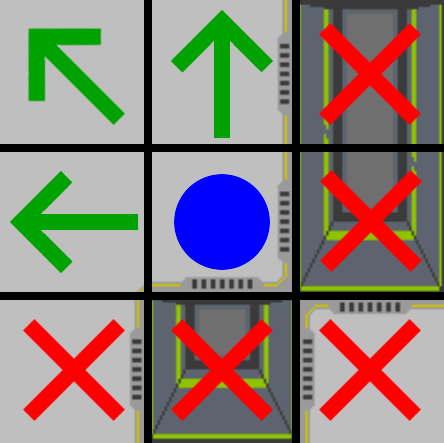
\includegraphics[width=0.4\linewidth]{pics/Graph_Generation.PNG}
 \captionof{figure}[Kalkulation der durch das Pfadfindesystems benutzbaren Levelteile]{Beispielhafte Darstellung der traversierbaren Nachbarteile ausgehend vom momentanen Levelteil (blau markiert) anhand eines Spielausschnitts. Nicht erreichbare Teile sind durch ein rotes Kreuz markiert.}
	\label{fig:graphNeighbourTiles}
\end{figure}

Bei der Berechnung, welche Levelteile durch die \texttt{GetConnectedNavPoints(...)}-Methode als begehbare Nachbarteile zurückgegeben werden, wird die \texttt{IsTraversable()} Funktion des gemeinsamen \texttt{ILevelTile}-Interfaces (siehe Abbildung \ref{fig:level_structure}) aller Levelteile verwendet. Prinzipiell sind alle direkt orthogonal oder diagonal verbundenen Levelteile potenzielle Nachbarn eines Teils, jedoch werden nicht traversierbare herausgefiltert, wie in Abbildung \ref{fig:graphNeighbourTiles} beispielhaft zu sehen ist. Bei diagonal verbundenen Nachbarteilen müssen zudem alle anliegenden orthogonalen Nachbarteile traversierbar sein, ansonsten werden diese Teile ebenfalls ausgeschlossen. Dies ist in Abbildung \ref{fig:graphNeighbourTiles} rechts und links unten beispielhaft zu sehen. Würden diese als begehbar bewertet werden, könnten später berechnete Laufpfade theoretisch direkt an Kanten von Wänden oder ähnlichem verlaufen, wodurch Gegner beim Versuch durch diese zu laufen daran stecken bleiben könnten.

Der Grund, weshalb die Abbildung des Levels als Graph in dieser Form realisiert wird, ist insbesondere, dass so vor Ausführung des Algorithmus nicht a priori ein entsprechender als Eingabe dienender Graph generiert werden muss. Zusätzlich ist dieser Ansatz flexibler gegenüber Änderungen im Level, weil die Nachbarschaftsbeziehungen von Levelteilen erst während der Pfadberechnungen ermittelt werden. Würde der Graph vorher generiert werden, müsste dieser hingegen bei jeder relevanten Änderung aktualisiert werden. Ein mögliches Problem der Kalkulation der verbundenen Graphknoten zur Laufzeit wäre, wenn diese Operation sehr aufwendig zu berechnen ist. In diesem Fall wäre eine vorherige Erzeugung des Graphen der bessere Ansatz. Tatsächlich lassen sich die traversierbaren Nachbarteile mit einer Worst-Case-Laufzeit von \textit{O(1)} berechnen, da die Anzahl möglicher Nachbarteile auf acht begrenzt ist und der Zugriff auf diese ebenso effizient möglich ist. Folglich ist es kein Problem die \texttt{GetConnectedNavPoints(...)}-Methode auch vielfach pro Pfadberechnung aufzurufen.

Das \texttt{NavMesh2D} stellt schließlich über die Methode \texttt{GetPathTo(...)} die Funktionalität zur Berechnung eines Pfades zwischen einem Start- und Endpunkt zur Verfügung. Diese wird zum einen intern zur Neukalkulation der Pfade der registrierten Agenten verwendet und kann zudem auch von externen Komponenten, wie zum Beispiel dem in Kapitel \ref{sec:audiosystem} näher beschriebenen Audiosystem, genutzt werden. Im Gegensatz zum eigentlichen Pfadfindungsalgorithmus liefert das \texttt{NavMesh2D} auch keine Liste von Levelteilen, sondern zweidimensionaler Vektoren als Pfad zurück. Dies liegt in erster Linie daran, dass die Levelteile, wie vorher beschrieben, als Graph für den Algorithmus dienen, die Agenten aber tatsächliche Weltkoordinaten in Form der Vektoren direkt zum Ablaufen der Pfade weiterverwenden können. Intern ruft das \texttt{NavMesh2D} also erst den Wegfindungsalgorithmus vom Levelteil am Startpunkt zum Teil am Endpunkt auf und konvertiert die Liste von Levelteilen schließlich in Weltkoordinaten. Abschließend werden der eigentliche Start- und Endpunkt wieder am generierten Pfad eingefügt und dieser, wie in Abschnitt \ref{sec:pathProcessing} beschrieben, mit dem \texttt{pathProcessor} nachbearbeitet. Der Wegfindealgorithmus liefert also zusammenfassend nur einen Rohpfad, der dann erst für die Weiterverwendung angepasst wird.

Außerdem verfügt das \texttt{NavMesh2D} noch über einen Zwischenspeicher für bereits berechnete Pfade in Form eines \texttt{PathCache}. Dieser dient vor allem dazu, häufige und kostenaufwendige Neukalkulationen von Wegen zu minimieren. Die exakte Funktionsweise wird in Abschnitt \ref{sec:pathCaching} allerdings noch genauer erläutert.

\subsubsection{Umsetzung des Pfadfindealgorithmus}\label{sec:pathfindingAlgo}
Der wichtigste Part des Navigationssystems ist im Kern der Pfandfindealgorithmus. Zwar stellt das \texttt{NavMesh2D} hierzu den Graphen zur Verfügung, jedoch muss durch den Algorithmus noch kalkuliert werden, wie ein Pfad zwischen einem gegebenem Start- und Endpunkt konkret verläuft. Klassischerweise wird zu diesem Zwecke der kürzeste Weg zwischen den beiden Punkten ermittelt.

Für diese Problemstellung existieren zwar zahlreiche Algorithmen, allerdings ist die Effizienz dieser für die Performanz des Spiels von ausschlaggebender Bedeutung, da die Berechnung kürzester Wege zumindest CPU-seitig zu den aufwendigeren Operationen zählt. Außerdem müssen die Pfade im ungünstigsten Fall für viele Gegner gleichzeitig ermittelt, und in kurzen Intervallen neu kalkuliert werden.

Zur Lösung dieser Probleme wird hierzu, vor allem auch in der Videospielentwicklung, sehr häufig der sogenannte \textit{A-Star Algorithmus} \cite{A_Star_Paper} angewendet. Dieser ist zwar prinzipiell nicht zwangs\-läu\-fig schneller, als zum Beispiel \textit{Dijkstras Algorithmus} \cite[658]{cormen}, kann aber in der realen Anwendung oft eine deutliche Beschleunigung bei Pfadberechnungen erzielen. Grund hierfür ist, dass A-Star folgende Voraussetzungen bei der Kalkulation gezielt ausnutzt:
\begin{itemize}
	\item Es existiert nur ein konkretes, bekanntes Ziel, zu dem der kürzeste Weg ermittelt werden soll.
	\item Die geschätzten Kosten zum Ziel lassen sich effizient von jedem Graphknoten aus berechnen.
\end{itemize}
Im Kern funktioniert der A-Star Algorithmus sehr ähnlich zu Dijkstras Algorithmus. Es werden vom aktuellen Knoten ausgehend Schrittweise jeweils die Nachbarknoten darauf untersucht, ob der Weg zu diesem Knoten kürzer ist, als der vorher eingetragene. Ist der untersuchte Knoten der Zielknoten, wird die Suche abgebrochen und der Weg zum Zielknoten zurückgegeben. Die als nächstes zu betrachtenden Knoten werden in einer Prioritätswarteschlange nach ihrer Distanz vom Startknoten aufsteigend eingeordnet und in dieser Reihenfolge durch den Algorithmus untersucht. Dies ist der Punkt, in dem der A-Star Algorithmus in der Vorgehensweise hauptsächlich von Dijkstras Algorithmus divergiert. Hier werden in der Prioritätswarteschlange die Kosten zu diesem Knoten plus die geschätzten Kosten zum Zielknoten verwendet (siehe \cite[S. 102]{A_Star_Paper}). Konkret bedeutet dies, dass bei A-Star neben Knoten, die möglichst nah am Startknoten liegen, außerdem auch Knoten, die geschätzt eine kurze Distanz zum Zielknoten haben, bevorzugt untersucht werden. Während Dijkstras Algorithmus also einfach stückweise die günstigsten Wege unabhängig von deren Richtung ermittelt, bis der Zielknoten erreicht ist, arbeitet A-Star von Anfang an zielgerichtet und kann so in den meisten Fällen die Zahl der benötigten Operationen deutlich verringern, obwohl es sich nach wie vor um einen Greedy-Algorithmus handelt. Dies ermöglicht A-Star innerhalb dieses Spiels zum Beispiel auf Flächen ohne Obstruktionen sofort einen kürzesten Weg zu finden, ohne unnötige Knoten innerhalb des Algorithmus zu expandieren.

Der entscheidende Faktor, ob der A-Star Algorithmus verwendet werden kann, beziehungsweise wie effizient dieser funktioniert, ist die sogenannte \textit{Heuristik}, die verwendet wird, um die Distanz von einem Knoten zum Zielknoten zu schätzen. Neben der bereits vorher genannten Anforderung, dass die Schätzung effizient durchgeführt werden können muss, sind folgende weitere Kriterien zu berücksichtigen:
\begin{itemize}
	\item Für keinen Knoten dürfen die geschätzten Kosten zum Ziel größer als die geschätzten Kosten eines Nachbarknotens zum Zielknoten plus die Kosten zu diesem Nachbarknoten sein \cite[S. 98]{ai_modern_approach}. Dies wird in der Heuristik auch \textit{Konsistenzkriterium} genannt. Ist dieses nicht erfüllt, ist auch das Optimalitätskriterium für den Algorithmus nicht mehr gegeben, was bedeutet, dass der Algorithmus bei Existenz eines Weges zum Ziel zwar terminiert, aber nicht zwangsläufig den kürzesten Weg zurückgibt.
	\item Die Heuristik sollte die Kosten im Optimalfall so schätzen, dass die Differenz zu den realen Kosten möglichst gering ist, denn durch eine genauere Schätzung sind im Durchschnitt weniger Rechenschnitte notwendig \cite[S. 98]{ai_modern_approach}.
\end{itemize}
Eine vor allem in der Spielentwicklung beliebte Heuristik ist die euklidische Distanz zwischen zwei Punkten, da die Navigation meist ohnehin in einem geometrischen Raum ausgeführt wird und die euklidische Distanz ein zuverlässiger Indikator für den Mindestabstand einer Verbindung zwischen zwei Punkten ist. Zudem erfüllt diese Heuristik aufgrund der Gültigkeit der Dreiecksungleichung im geometrischen Raum das Konsistenzkriterium und ist zudem schnell mit Laufzeit \textit{O(1)} durch die Berechnung des Abstands zweier Vektoren ermittelbar. Aus den genannten Gründen wird die euklidische Heuristik auch innerhalb dieses Projekts für den A-Star Algorithmus eingesetzt.

Für die Prioritätswarteschlange, in der die als nächstes zu expandierenden Knoten gehalten werden, wurde ein Fibonacci-Heap implementiert. Der Grund für die Verwendung dieser speziellen Form eines Heaps ist, dass dieser eine Laufzeit für das Einfügen neuer Elemente von \textit{O(1)} bietet \cite[S. 511]{cormen}, im Gegensatz zu \textit{O(log(n))} beispielsweise bei einem binären Heap \cite[S. 164]{cormen}. Dies ist in diesem Fall insofern relevant, dass jedes Teil im Level bis zu acht begehbare Nachbarteile besitzen kann, welche in den Heap eingefügt werden müssen. Ebenso kann in einem Fibonacci-Heap der Schlüssel eines Elements in konstanter Laufzeit verringert werden \cite[S. 518]{cormen}, was beim A-Star Algorithmus konkret bei der Relaxierung von Kanten geschieht. Tatsächlich ist dieser theoretische Vorteil hier nahezu irrelevant, da aufgrund der Gültigkeit der Dreiecksungleichung der direkte Weg zwischen zwei Knoten auch immer der Kürzeste ist, was de-facto dazu führt, dass keine Kanten zu einem Knoten relaxiert werden, nachdem das erste Mal ein kürzester Weg zu diesem gefunden wurde. Aufgrund der schnellen Laufzeit beim Einfügen von Elementen bietet sich ein Fibonacci-Heap dennoch als Datenstruktur an. Nebenbei ist anzumerken, dass das Entfernen des Minimums aus dem Fibonacci-Heap theoretisch ein Problem für die Performanz sein könnte, da nur in der amortisierten Analyse eine sehr schnelle Laufzeit von \textit{O(log(n))} gegeben ist. Das bedeutet, dass diese Operation in Ausnahmefällen auch eine deutlich schlechtere Zeitkomplexität hat, was zu einem unflüssigen Spielerlebnis führen könnte. In der realen Anwendung sind solche Performanzeinbrüche jedoch nicht zu beobachten, auch wenn mehrere längere Pfade berechnet werden müssen.

\subsubsection{Pfadverarbeitung für die Verwendung bei den Gegnern}\label{sec:pathProcessing}
Mithilfe des A-Star Algorithmus lassen sich soweit effizient auf Levelteilen basierend kürzeste Pfade berechnen, jedoch lassen sich diese durch entsprechende Nachbearbeitung besser durch die Navigationsagenten nutzen. Aktuell führt das \texttt{NavMesh2D} folgende zwei Bearbeitungsschritte durch:
\begin{itemize}
	\item Entfernen von \textit{Backtracking} (siehe Abbildung \ref{fig:backtrackingPath}) am Start und Ende des Pfades.
	\item Entfernen unnötiger Pfadpunkte. Dies sind Wegpunkte, die auf einer direkten Linie zwischen zwei anderen Pfadpunkten liegen, und somit keine zusätzliche relevante Information zur Navigation darstellen.
\end{itemize}

\begin{figure}[h]
 \centering
 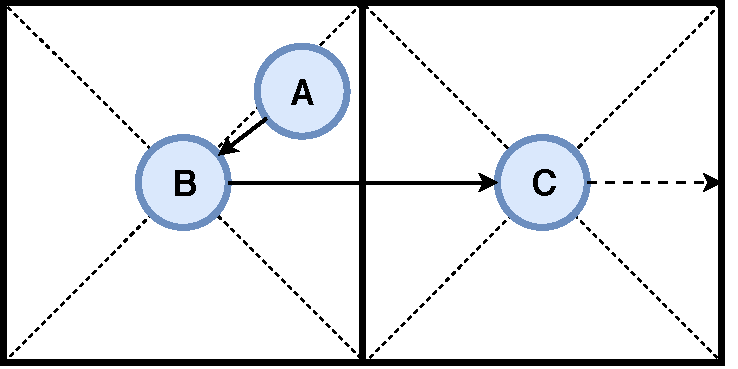
\includegraphics[width=0.4\linewidth]{pics/Backtracking_Example.pdf}
 \captionof{figure}[Beispiel für \textit{Backtracking} am Anfang eines Pfades]{Beispiel für \textit{Backtracking} am Anfang eines Pfades zwischen den Punkten A, B und C.}
	\label{fig:backtrackingPath}
\end{figure}

Erstere Operation ist vonnöten, da der tatsächliche Start- und Endpunkt des Pfades nach Berechnung des teilebasierten Pfades noch eingefügt wird. Dies kann dazu führen, dass zum Beispiel am Start ein Pfad zurückführt, obwohl dieser dann in eine andere Richtung verläuft, wie beispielhaft in Abbildung \ref{fig:backtrackingPath} zu sehen. Dort ist der Punkt A der tatsächliche Startpunkt, während Punkt B und C teil des vom Pfadfindealgorithmus kalkulierten Pfades sind. In einem solchen Fall wird der mittlere Knoten, also hier B, aus dem Pfad entfernt, um beim Agenten später unnötige Bewegungen zu vermeiden. Am Ende des Pfades wird analog verfahren.

\begin{figure}[h]
 \centering
 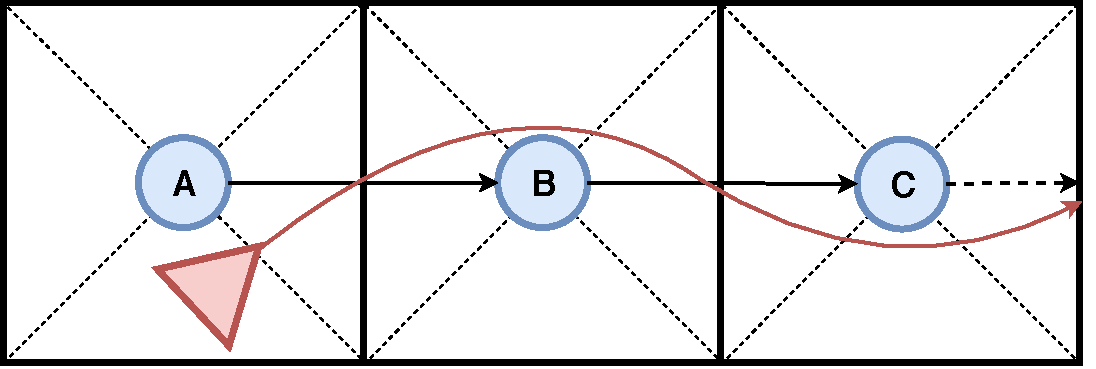
\includegraphics[width=0.6\linewidth]{pics/Enemy_Path_Oscillation.pdf}
 \captionof{figure}[Oszillierende Pfadabweichung von Gegnern bei vielen Pfadpunkten]{Beispielhafte Darstellung der oszillierenden Pfadabweichung von Gegnern (rot dargestellt) auf einem geraden Pfad mit vielen Knotenpunkten.}
	\label{fig:enemyOscillation}
\end{figure}

Die zweite genannte Pfadnachbearbeitung führt ebenso zu einem besseren Bewegungsverhalten bei den Agenten. Das grundlegende Problem ist, dass die Agenten durch die Anwendung physikalischer Kräfte bewegt werden und so in der Bewegung träge sind. Dies ist zwar prinzipiell bewusst so gewählt, um die Bewegung flüssig erscheinen zu lassen, jedoch bleibt zum Beispiel auf einer geraden Strecke die laterale Geschwindigkeit erhalten. Das bedeutet, dass der Agent sich beim Ablaufen des Pfades zwischen den Pfadpunkten seitlich hin- und herbewegen kann, wie in Abbildung \ref{fig:enemyOscillation} skizziert ist. Der beschriebene Effekt ist zwar nur subtil, lässt die Bewegung der Agenten allerdings unnatürlich aussehen. Durch die Entfernung unnötiger Pfadpunkte (in der Abbildung entspricht dies B) lässt sich dieser Effekt vermeiden und der Pfad an sich wird ohne relevanten Informationsverlust vereinfacht.

Beide der genannten Pfadverarbeitungsoperationen könnten theoretisch in Form von Methoden des \texttt{NavMesh2D} realisiert werden. Um eine bessere Wiederverwendbarkeit und Flexibilität des Systems zu gewährleisten, wird die Pfadbearbeitung jedoch mithilfe des \textit{Decorator}-Entwurfsmusters \cite[175]{Design_Patterns} umgesetzt. Jede Klasse die das \texttt{IPathProcessor} Interface implementiert (siehe Abbildung \ref{fig:pathfinding_structure}), kann über den Konstruktor einen weiteren \texttt{IPathProcessor} übergeben bekommen. Bei Aufruf der \texttt{ProcessPath(...)}-Methode wird dann erst die selbe Methode beim übergebenen \texttt{IPathProcessor} aufgerufen, sofern vorhanden. So kann ein Pfadverarbeiter individuell konfiguriert werden. Das \texttt{NavMesh2D} erzeugt schließlich beim Start der Spielszene einen entsprechenden Pfadverarbeiter, der dann auf allen vom Wegfindealgorithmus errechneten Pfaden angewandt wird.

\subsubsection{Pfadspeicherung zur Performanzverbesserung}\label{sec:pathCaching}
Durch Verwendung des A-Star Algorithmus in Kombination mit Fibonacci-Heaps lassen sich Pfadberechnungen bereits sehr performant durchführen. Dennoch ist es sinnvoll die Effizienz wenn möglich weiter zu verbessern, da in keiner Weise festgelegt ist, wie viele Gegner gleichzeitig pro Level aktiv sein können. Folglich lässt sich aus einer guten Performanz in den getesteten Leveln kein allgemeiner Schluss ziehen. Deshalb wird zusätzlich ein Pfadspeicherungssystem integriert, welches vom \texttt{NavMesh2D} genutzt wird und kürzlich berechnete Pfade zwischenspeichert.

Der in Abbildung \ref{fig:pathfinding_structure} dargestellte \texttt{PathCache} wird bei Start der Spielszene durch das \texttt{NavMesh2D} erzeugt. Dabei wird im Konstruktor die maximale Anzahl gleichzeitig zwischengespeicherter Pfade spezifiziert. Der Speicher an sich ist durch ein zweifach verschachteltes \texttt{Dictionary} umgesetzt, bei dem das Start- und Endteil des Pfades jeweils den Schlüssel darstellen und der Pfad an sich den Wert des inneren \texttt{Dictionary}. Dies ermöglicht die Abfrage von Pfaden mit der \texttt{TryGetPath(...)}-Methode in konstanter Laufzeit über je eine Hash-Suche des Start- und Endpunktes. Über die \texttt{CachePath(...)}-Methode lassen sich Pfade zum Speicher hinzufügen. Gegensätzlich lassen sich durch Aufruf von \texttt{InvalidateCache(...)} Wege wieder aus dem Speicher entfernen.

Ein Problem des Systems ist, dass die Anzahl möglicher Pfade quadratisch mit der Anzahl an Levelteilen wächst. Würden also alle berechneten Pfade gespeichert werden, würde dies rasch eine substanzielle Menge an Arbeitsspeicher in Anspruch nehmen. Deshalb wird bei erreichen der Speicherkapazität \texttt{maxSize} bei Speicherung eines Pfades ein anderer nach dem Prinzip \textit{Least Recently Used} aus dem Pfadspeicher verdrängt. Zu diesem Zweck führt der \texttt{invalidationBuffer} mit, in welcher Reihenfolge die Pfade zuletzt verwendet wurden. Wird ein Weg aus dem Speicher abgefragt, wird dieser wieder an den Anfang des Puffers gesetzt. Bei Überschreitung der Maximalgröße wird dann das letzte Element entfernt. Die Pfade werden im \texttt{invalidationBuffer} als Tupel aus Start- und Endpunkt gehalten.

Das \texttt{NavMesh2D} prüft nun vor der Pfadberechnung erst, ob der gesuchte Pfad bereits im Speicher ist. Nur wenn dies nicht der Fall ist, wird tatsächlich der Wegfindealgorithmus aufgerufen und das Ergebnis schließlich im \texttt{PathCache} abgelegt. So lassen sich durch geringfügig höheren Arbeitsspeicherverbrauch viele aufwendige Pfadberechnungen verhindern. Vor allem die Wege zwischen den Patroullienpunkten von Gegnern müssen so in der Regel nur ein einziges Mal bei Levelstart kalkuliert werden und sind von diesem Zeitpunkt an im Speicher abgelegt.

\subsubsection{Integration des Wegfindungssystems in das Gegnerverhalten}\label{sec:pathfindingIntegration}
Nachdem das Pfadfindungssystem soweit funktional und effizient ist, muss es schließlich noch in die Gegner integriert werden. Hierzu hat jeder Gegner eine \texttt{NavAgent}-Komponente. Diese wird standardmäßig genutzt, um die Patrouillienpunkte abzulaufen, indem immer der Nächste als aktuelles Ziel des Agenten gesetzt wird.

\begin{figure}[h]
 \centering
 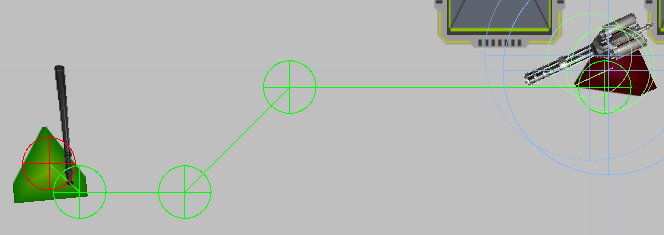
\includegraphics[width=0.7\linewidth]{pics/path_gizmo.png}
 \captionof{figure}[Debug-Anzeige für Gegnerpfade]{Debug-Anzeige des aktuellen Pfades eines Gegners. Die Pfadpunkte werden dabei als Kreise dargestellt.}
	\label{fig:pathGizmo}
\end{figure}

 Um das Debuggen zu erleichtern, werden die aktuellen Routen der Gegner bei Auswahl in der Szene als sogenannte \textit{Gizmo}s angezeigt. Dies sind Elemente, die nur innerhalb des Unity Editors angezeigt werden können, um zusätzliche visuelle Information zu Spielobjekten zu erhalten. In Abbildung \ref{fig:pathGizmo} ist die Debug-Ansicht eines Gegnerpfades beispielhaft abgebildet.

Neben dem Ablaufen von Patrouillienpunkten ist das Verhalten der Gegner, sobald der Spieler entdeckt wurde, deutlich komplexer. In diesem Fall soll der Spieler verfolgt werden und solange die Aufmerksamkeit der Gegner über dem Angriffsschwellwert liegt, gegebenenfalls aktiv gesucht werden. Da das Suchverhalten der Gegner von Typ zu Typ variieren soll, wird hierfür das Decorator-Entwurfsmuster \cite[175]{Design_Patterns} eingesetzt, wie in Abbildung \ref{fig:followBehaviourUML} dargestellt. So wird verhindert, dass für jeden Gegnertyp eine Unterklasse mit individuellem Verhaltensmuster erstellt werden muss. Stattdessen wird das Verhalten bei Erzeugung der Gegner erstellt und diesen schließlich zugewiesen und kann so je nach Typ konfiguriert werden.

\begin{figure}[h]
 \centering
 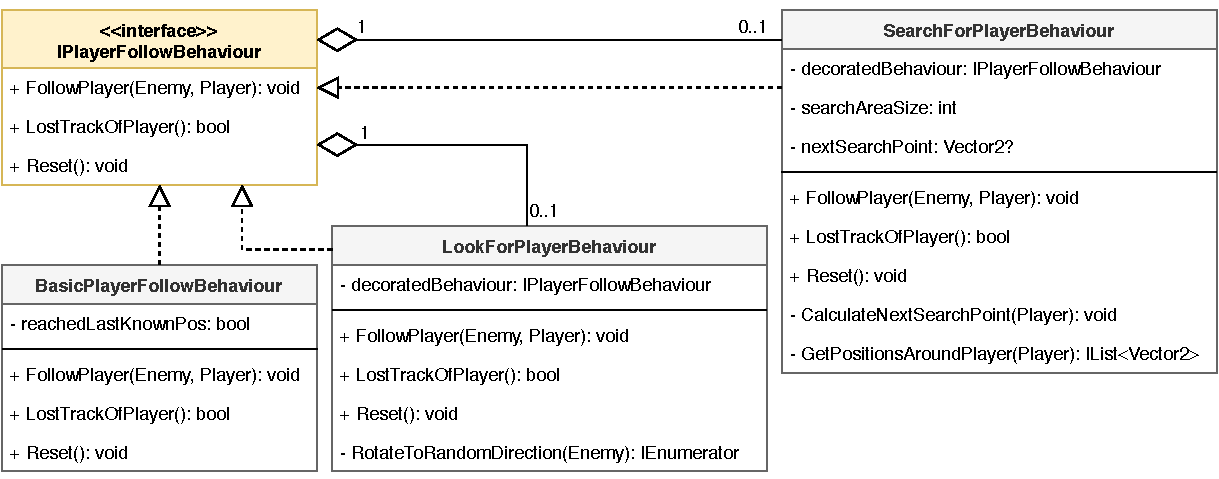
\includegraphics[width=1\linewidth]{diagrams/Player_Follow_Behaviour_UML.pdf}
 \captionof{figure}[Decorator für das Spieler-Suchverhalten der Gegner]{UML-Diagramm für das Spieler-Suchverhalten der Gegner.}
	\label{fig:followBehaviourUML}
\end{figure}

Das Interface für das Verfolgungs- beziehungsweise Suchverhalten der Gegner beinhaltet folgende drei Grundfunktionen, die durch alle Unterklassen implementiert werden müssen:

\begin{itemize}
	\item\textbf{\texttt{FollowPlayer(...)}:} Signalisiert der Verhaltensklasse, dass der Gegner dem Spieler folgen soll. Diese Methode wird zyklisch durch den Gegner aufgerufen, solange dessen Aufmerksamkeitslevel über dem Angriffsschwellwert ist.
	\item\textbf{\texttt{LostTrackOfPlayer()}:} Diese Methode gibt einen boolschen Wert zurück der angibt, ob der Gegner die Spur des Spielers verloren hat.
	\item\textbf{\texttt{Reset()}:} Diese Methode wird durch den Gegner aufgerufen, sobald dieser wieder zum Normalverhalten zurückkehrt und kann durch die konkreten Verhaltensklassen genutzt werden, um sich auf den Anfangszustand zurückzusetzen.
\end{itemize}

Alle Unterklassen, abgesehen vom \texttt{BasicPlayerFollowBehaviour}, müssen innerhalb der Inter\-face-Methoden jeweils auch die Methode des dekorierten Verhaltens aufrufen. So lässt sich das Verhalten durch jede spezifische Implementierung stückweise erweitern, ohne die Funktionalität der anderen abzuändern.

Das \texttt{BasicPlayerFollowBehaviour} ist der Grundbaustein für das Suchverhalten aller Gegner. Es setzt im Agenten des Gegners die letzte bekannte Position des Spielers als Ziel und folgt diesem so direkt. Die letzte bekannte Position ist die Stelle, an der der Spieler zuletzt durch den Gegner gesehen oder gehört wurde. Sobald dieser Punkt erreicht ist, gibt die \texttt{LostTrackOfPlayer()}-Methode auch \texttt{true} als Rückgabewert zurück. Dies wird durch die anderen Verhaltensunterklassen als Signal gewertet, weitere Suchmaßnahmen einzuleiten.

Das \texttt{LookForPlayerBehaviour} lässt den Gegner schließlich nach Erreichen der letzten bekannten Spielerposition, randomisiert in verschiedene Richtungen blicken, um so zu versuchen erneuten Sichtkontakt zum Spieler wiederherzustellen. Die Koroutine \texttt{RotateToRandomDirection()} übernimmt dabei das Rotieren des Gegners.

Weil schwerere Gegner nach Verlust der Spur des Spieler zusätzlich noch aktiv die Umgebung absuchen sollen, wird zu diesem Zweck bei diesen noch das \texttt{SearchForPlayerBehaviour} eingesetzt. Bei der Umsetzung ist entscheidend, ob die Gegner tatsächlich direkt zum Spieler navigieren sollen, also de-facto immer dessen Position kennen, oder uninformiert und somit theoretisch realistischer die Gegend beispielsweise randomisiert absuchen sollen. Konkret wird eine Kompromisslösung aus den beiden Ansätzen gewählt, sodass Gegner mit diesem Suchverhalten nicht immer direkt zum Spieler laufen, aber trotzdem gezielt in dessen Nähe nach diesem suchen, um so eine Balance aus Realismus und Herausforderung zu schaffen. Hierzu wird im Umkreis um den Spieler zufällig ein begehbares Levelteil ausgewählt und als Ziel des Navigationsagenten des Gegners gesetzt. Bei Erreichen dieses Punktes wird solange erneut ein solcher zufälliger Punkt gewählt, bis das Aufmerksamkeitslevel des Gegners unter den Angriffsschwellwert fällt. Die \texttt{searchAreaSize} gibt an, in welchem Umkreis in Form von Teilen um den Spieler Suchpunkte ausgewählt werden können. Ein geringerer Wert bedeutet also, dass der Gegner zielgenauer nach dem Spieler sucht. Dies ermöglicht, dass die Gegner zwar durchaus aktiv und relativ zielgerichtet suchen, durch die Ungenauigkeit aber dem Spieler dennoch die Möglichkeit einräumen zu entkommen.